\documentclass[../main.tex]{subfiles}
\begin{document}

\subsection{QCD multi-jet}
\label{hh:subsec:qcd}


Generic QCD multi-jet events can enter the final selection if two jets are misidentified as the $\tau\tau$ pair. The process creating QCD multi-jets has the largest cross section among all the background processes so, event it gets reduced thanks to the analysis selections, its contribution ends up being notably important, particularly in the $\tau_h\tau_h$ channel. Estimating the QCD background contribution via simulated events would require a prohibitively large number of them, so the estimation is performed using a data-driven method. The strategy used is often called ``ABCD'' method, and is described as follows.


\subsubsection{QCD background estimation using the ABCD method}

The ABCD takes its name from the fact that four regions are used: the signal region, A, and three other regions, B, C and D, obtained by reverting two different selection criteria. In the \hhbbtt{} analysis, region A (\textit{opposite-sign, isolated}) requires that both leptons are isolated and have opposite sign. Region B (\textit{same-sign, isolated}) is obtained by inverting the tau pair charge requirement. In region C (\textit{opposite-sign, non-isolated}), the DeepTauVsJet selection is inverted by requiring that the selected $\tau_h$ (the one with the lowest $p_t$ in the $\tau_h\tau_h$ channel) fails the medium working point but still passes the VVVLoose one. Region D (\textit{same-sign, non-isolated}) combines these two inverted selections. An sketch of the four regions is shown in Fig.~\ref{hh:fig:qcd_sketch}.

\begin{figure}[h!]
\begin{center}
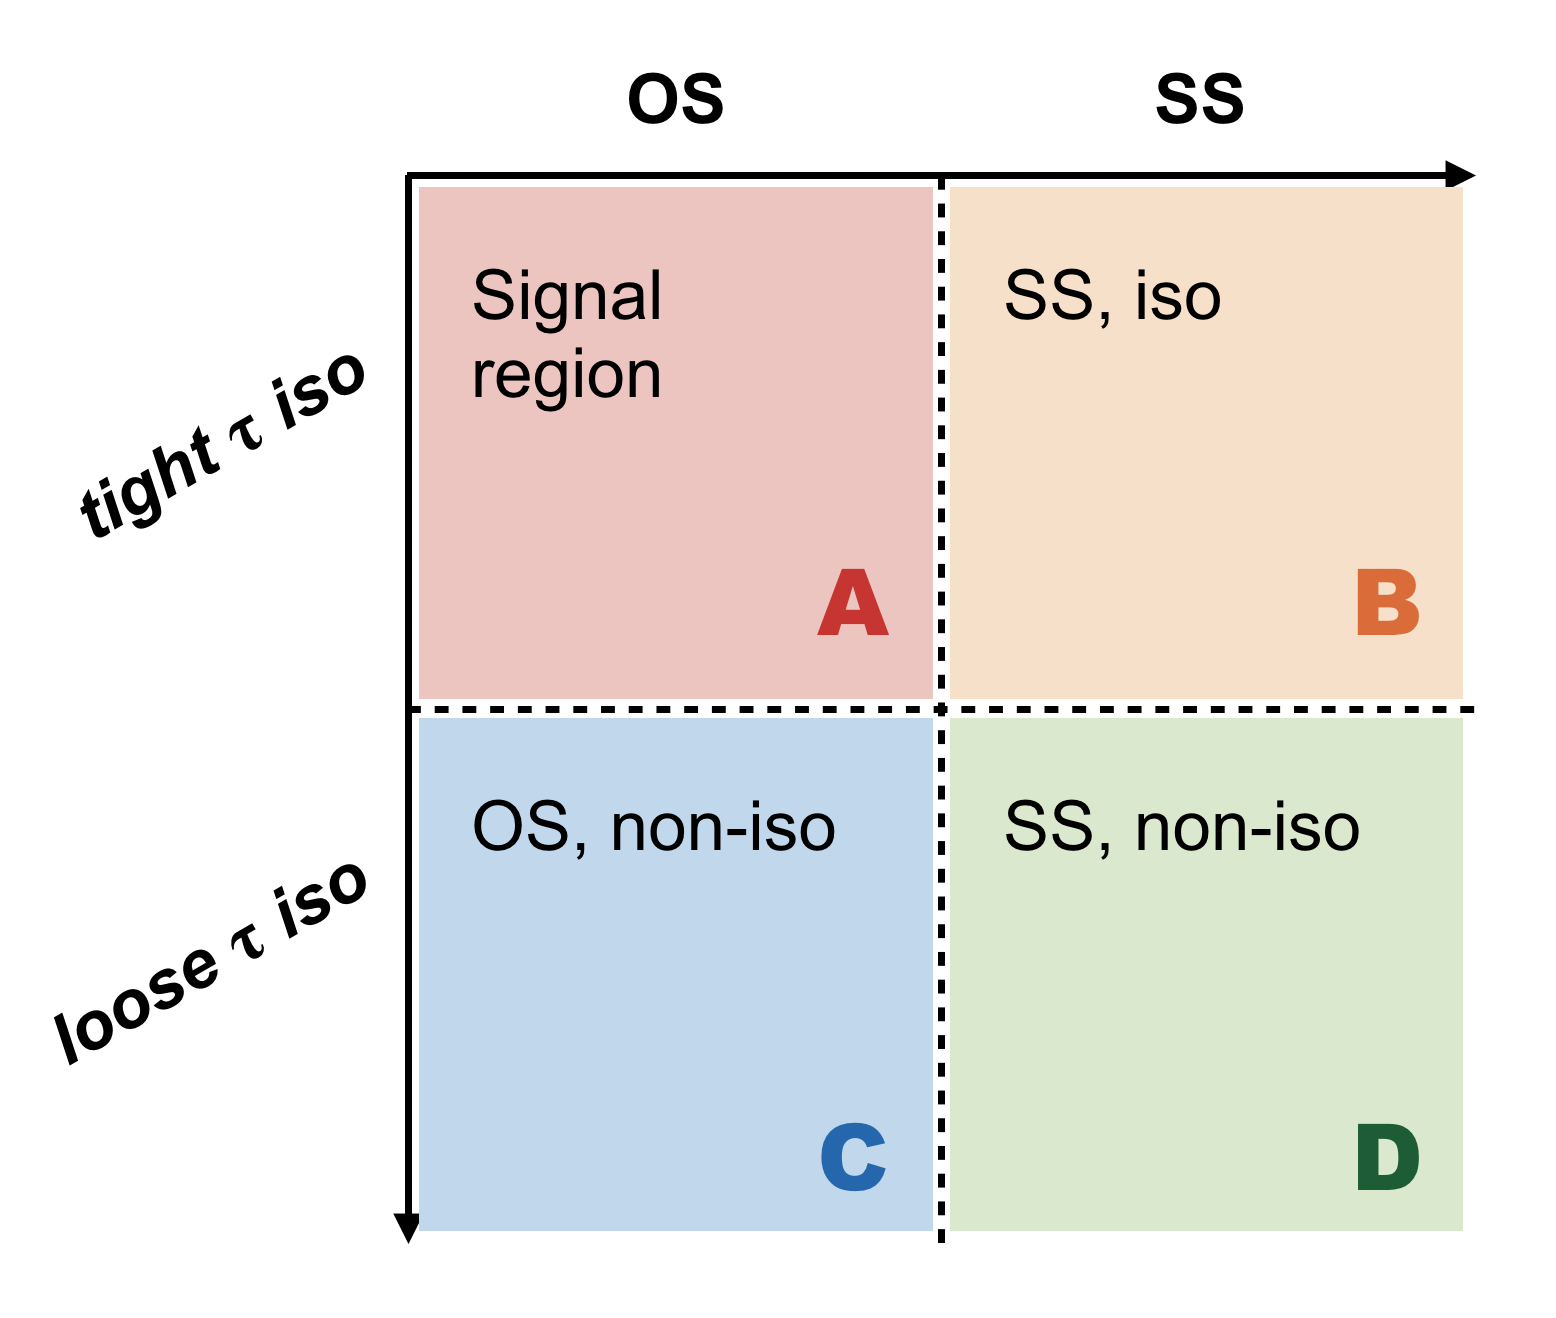
\includegraphics[width=0.5\textwidth]{Images/QCDschema}
\end{center}
\caption[ABCD method for QCD background estimation]{Sketch of the four regions used to estimate the QCD multi-jet background.}
\label{hh:fig:qcd_sketch}
\end{figure}

The distribution of the multi-jet QCD contribution in any given binned variable is estimated from the C region: yields from the other backgrounds are substracted from the data in this region and the remaining number of events in each bin is then multiplied by a factor $k^{\text{iso/non-iso}}$. This factor accounts for moving from the non-isolated selection (present in region C) to the isolated selection (used in the signal region), and is measured as the ratio of event yields in regions B and D after substracting the other background yields in each region. Therefore, the ABCD method gives a QCD estimation whose shape comes from region C and its yield from regions B, C and D as given by the formula C $\times$ B / D. However, in some analysis categories, due to the lack of statistics, a different selection is applied to regions B and D. In the boosted category, the B / D ratio is computed with all the selections defined in the category excluding the b-tagging requirement, while in the five VBF subcategories, the B / D correction factor is estimated from the VBF inclusive category, which includes the five subcategories.

Something to be noted is that the decision of considering region C to obtain the shape from the QCD distributions instead of region B is quite arbitrary. This decision will be discussed in Section~\ref{hh:sec:systematics}.






%\bibliographystyle{unsrt}
%\bibliography{../biblio.bib}



\end{document}

